% Sec. Ground Truth Without Motion Capture
% Sec. V Pose Reference Without Motion Capture (about 0.9 page).
\section{A Pose Reference Without Motion Capture}
\label{sec:gt}
This section answers how accurately the testbed knows where every
agent is, at building scale, using only onboard sensors. The result is a
reference, not survey-grade ground truth: each check below bounds one
of its errors, and absolute scale is fixed by the control distances. The reference
map is SLAM-derived, which removes the survey scanner normally required
for map registration; every scan is registered against it, so the pose
is carried by the map and not by odometry between anchors; and
fiducial boards posed in the map frame anchor the RGB-D cart and the
masts where registration alone is weak. Fig.~\ref{fig:refpipeline}
shows the pipeline.

\begin{figure*}[t]
\centering
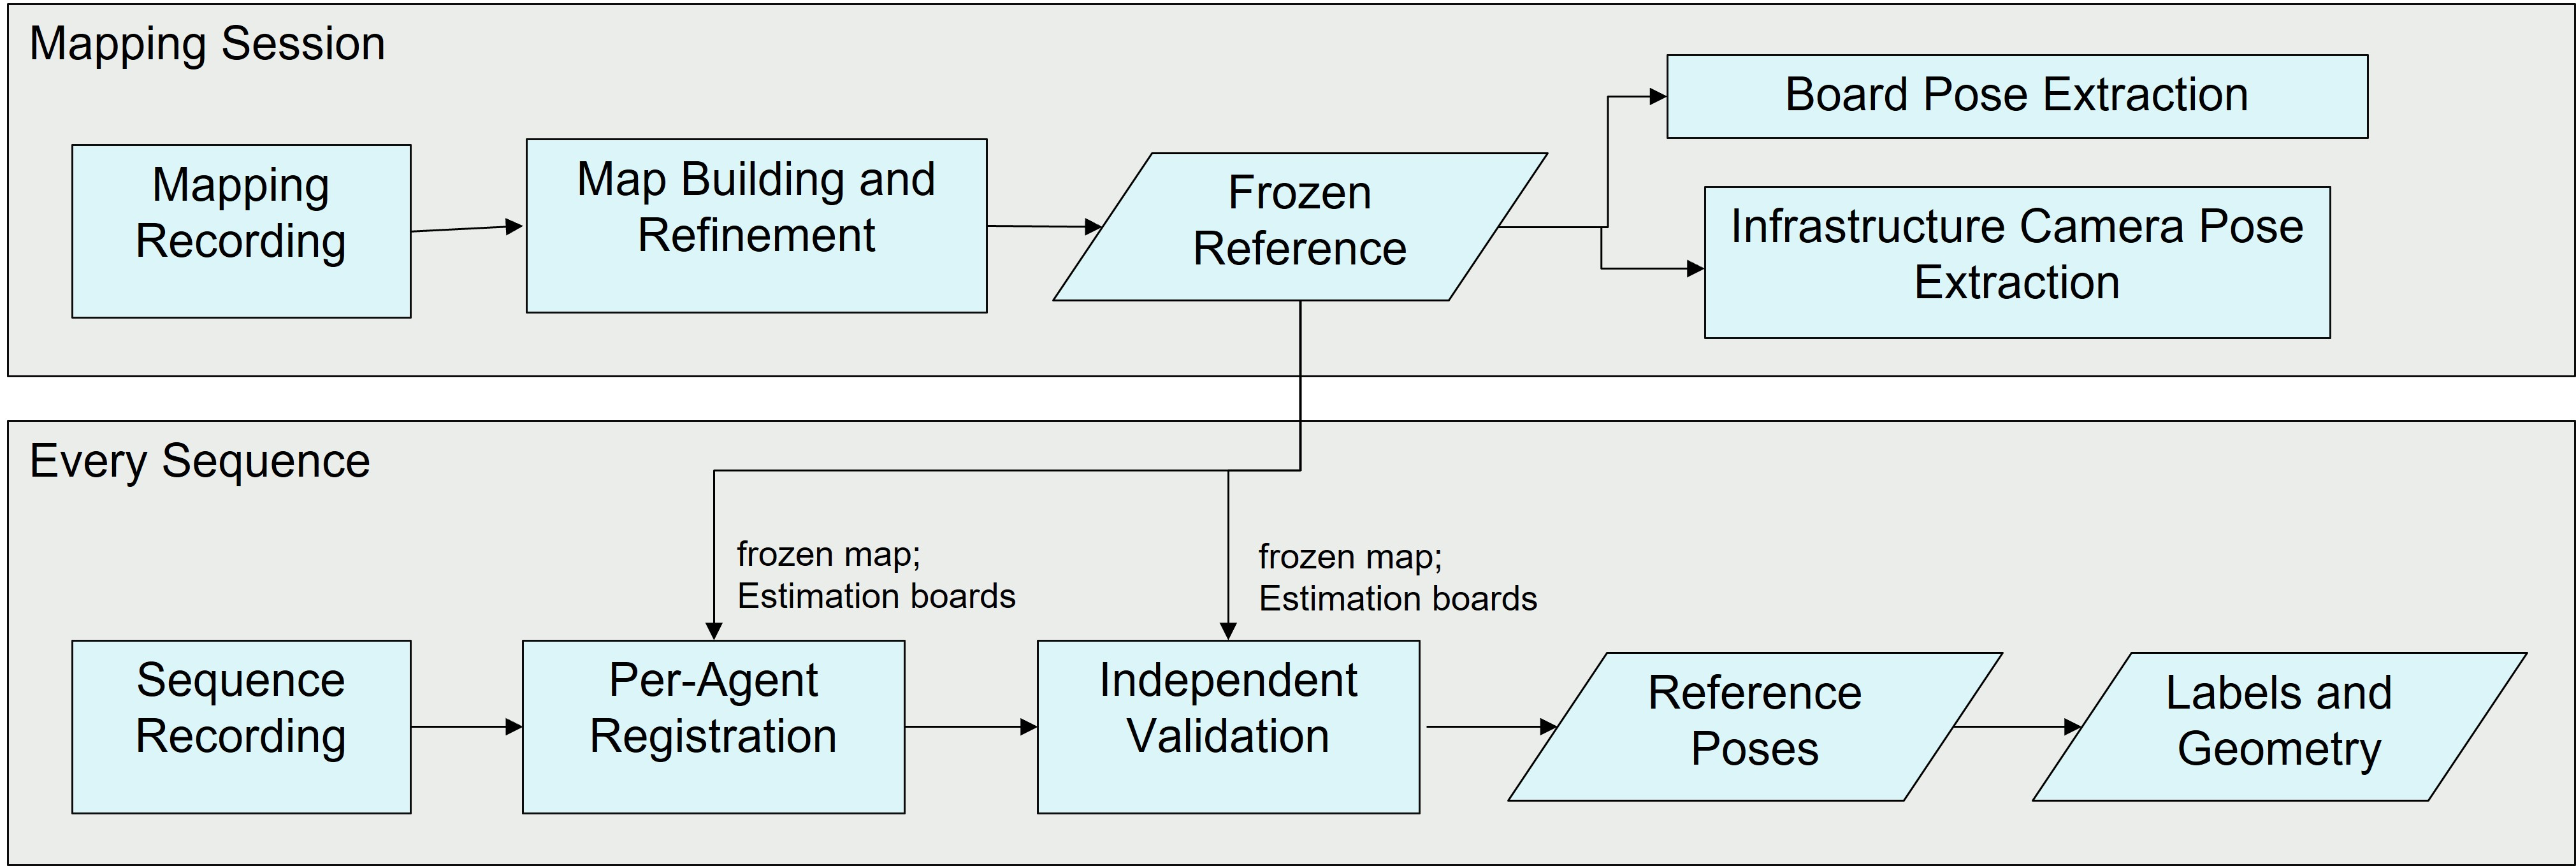
\includegraphics[width=\textwidth]{figs/fig_refpipeline.jpg}
\caption{Reference pipeline. Top: the mapping session, run once per
site, builds and refines the map, poses the boards in it
(Eq.~\eqref{eq:board_chain}), and places the infrastructure cameras
through the boards (Eq.~\eqref{eq:infra_camera_chain}). Bottom: each
sequence is registered into the frozen map, by scan-to-map ICP for the
LiDAR agents and by odometry with ICP and board factors for the RGB-D
agent, and the poses are exported in the site frame.}
\label{fig:refpipeline}
\end{figure*}

\subsection{Reference Map}
\label{sec:map}
% Sec. V-A "Reference Map" for main.tex, with the bundle-adjusted and
% TSDF-fused reference (pass 20261015). To use: replace the body of
% \subsection{Reference Map} in main.tex (from "The reference map is built"
% to "...would not be visible to conventional ICP.") with
% % Sec. V-A "Reference Map" for main.tex, with the bundle-adjusted and
% TSDF-fused reference (pass 20261015). To use: replace the body of
% \subsection{Reference Map} in main.tex (from "The reference map is built"
% to "...would not be visible to conventional ICP.") with
% % Sec. V-A "Reference Map" for main.tex, with the bundle-adjusted and
% TSDF-fused reference (pass 20261015). To use: replace the body of
% \subsection{Reference Map} in main.tex (from "The reference map is built"
% to "...would not be visible to conventional ICP.") with
% \input{sections/refmap_main}. Full method and equations:
% supplementary, supp/refmap_method.tex.
The reference map is built in a dedicated mapping session and held fixed
afterwards; no recorded run contributes to it. A LiDAR-inertial SLAM
solution \cite{glim} gives the initial trajectory. It is refined by plane
bundle adjustment \cite{balm,hba}: the poses of \SI{1}{\second} keyframes
are moved jointly so that every planar patch seen from several keyframes is
as thin as possible, the cost of a patch being the smallest eigenvalue of
the scatter of its points, with the SLAM solution's relative motion and
gravity direction kept as soft priors. The scans are then fused into a
truncated signed distance field \cite{curless1996,vdbfusion} with
\SI{2}{\centi\metre} cells and a truncation of \SI{8}{\centi\metre}, three
standard deviations of the spread with which the scans place a wall; the
map is its zero-level surface, and moving objects are removed by
free-space carving \cite{dufomap}. Fusion matters as much as the poses: the
usual union of points keeps every cell a stray point reached, which widened
walls by \SI{4}{\centi\metre} over the scans that built them, whereas the
signed distance averages across a surface. Each stage is measured by the
thickness of the map's planar surfaces (Table~\ref{tab:refmap_stages}):
from the SLAM solution alone to the reference, walls go from
\SI{14.3}{\centi\metre} to \todo{} and floors from \SI{3.6}{\centi\metre}
to \todo{}, and the doubled surfaces left by drift between visits fall
from 2.0\,\% to \todo{}. Against the reference, the SLAM trajectory's error
is a heading error of about $0.6^\circ$ that builds within
\SI{10}{\second} and does not grow further, with an ATE of \todo{}
(Table~\ref{tab:glim_vs_ref}). Bundle adjustment started from two
different trajectories reaches the same poses to \SI{0.7}{\centi\metre}
(median, after alignment) and $0.1^\circ$, so the result is fixed by the
scans and not by the starting point.
. Full method and equations:
% supplementary, supp/refmap_method.tex.
The reference map is built in a dedicated mapping session and held fixed
afterwards; no recorded run contributes to it. A LiDAR-inertial SLAM
solution \cite{glim} gives the initial trajectory. It is refined by plane
bundle adjustment \cite{balm,hba}: the poses of \SI{1}{\second} keyframes
are moved jointly so that every planar patch seen from several keyframes is
as thin as possible, the cost of a patch being the smallest eigenvalue of
the scatter of its points, with the SLAM solution's relative motion and
gravity direction kept as soft priors. The scans are then fused into a
truncated signed distance field \cite{curless1996,vdbfusion} with
\SI{2}{\centi\metre} cells and a truncation of \SI{8}{\centi\metre}, three
standard deviations of the spread with which the scans place a wall; the
map is its zero-level surface, and moving objects are removed by
free-space carving \cite{dufomap}. Fusion matters as much as the poses: the
usual union of points keeps every cell a stray point reached, which widened
walls by \SI{4}{\centi\metre} over the scans that built them, whereas the
signed distance averages across a surface. Each stage is measured by the
thickness of the map's planar surfaces (Table~\ref{tab:refmap_stages}):
from the SLAM solution alone to the reference, walls go from
\SI{14.3}{\centi\metre} to \todo{} and floors from \SI{3.6}{\centi\metre}
to \todo{}, and the doubled surfaces left by drift between visits fall
from 2.0\,\% to \todo{}. Against the reference, the SLAM trajectory's error
is a heading error of about $0.6^\circ$ that builds within
\SI{10}{\second} and does not grow further, with an ATE of \todo{}
(Table~\ref{tab:glim_vs_ref}). Bundle adjustment started from two
different trajectories reaches the same poses to \SI{0.7}{\centi\metre}
(median, after alignment) and $0.1^\circ$, so the result is fixed by the
scans and not by the starting point.
. Full method and equations:
% supplementary, supp/refmap_method.tex.
The reference map is built in a dedicated mapping session and held fixed
afterwards; no recorded run contributes to it. A LiDAR-inertial SLAM
solution \cite{glim} gives the initial trajectory. It is refined by plane
bundle adjustment \cite{balm,hba}: the poses of \SI{1}{\second} keyframes
are moved jointly so that every planar patch seen from several keyframes is
as thin as possible, the cost of a patch being the smallest eigenvalue of
the scatter of its points, with the SLAM solution's relative motion and
gravity direction kept as soft priors. The scans are then fused into a
truncated signed distance field \cite{curless1996,vdbfusion} with
\SI{2}{\centi\metre} cells and a truncation of \SI{8}{\centi\metre}, three
standard deviations of the spread with which the scans place a wall; the
map is its zero-level surface, and moving objects are removed by
free-space carving \cite{dufomap}. Fusion matters as much as the poses: the
usual union of points keeps every cell a stray point reached, which widened
walls by \SI{4}{\centi\metre} over the scans that built them, whereas the
signed distance averages across a surface. Each stage is measured by the
thickness of the map's planar surfaces (Table~\ref{tab:refmap_stages}):
from the SLAM solution alone to the reference, walls go from
\SI{14.3}{\centi\metre} to \todo{} and floors from \SI{3.6}{\centi\metre}
to \todo{}, and the doubled surfaces left by drift between visits fall
from 2.0\,\% to \todo{}. Against the reference, the SLAM trajectory's error
is a heading error of about $0.6^\circ$ that builds within
\SI{10}{\second} and does not grow further, with an ATE of \todo{}
(Table~\ref{tab:glim_vs_ref}). Bundle adjustment started from two
different trajectories reaches the same poses to \SI{0.7}{\centi\metre}
(median, after alignment) and $0.1^\circ$, so the result is fixed by the
scans and not by the starting point.


\paragraph{A coloured mesh.} The zero-level surface of the signed
distance field is extracted as a mesh, and its colours come from a 3D
Gaussian splatting model \cite{kerbl2023gaussian} trained on the
mapping session's camera images at their reference poses
\unsure{state how the splats' colours are transferred to the mesh
vertices or faces}. The same map is thus a metric reference for poses
and an appearance reference for rendering: a view rendered from it at a
held-out camera pose can be compared with the image that camera
recorded, \todo{PSNR / SSIM / LPIPS on held-out views}.

The frozen map is the metric backbone of every run. LiDAR agents are
localized by scan-to-map registration. For \texttt{mobile\_2}, depth
registration, visual odometry, and a subset of the board sightings of
Sec.~\ref{sec:fiducials} are combined in one pose-graph optimization
per run, with the selected boards entering as absolute pose factors;
the remaining boards are held out for validation. The LiDAR agents
need no board factors, so for them every board sighting is a
validation measurement. All trajectories therefore share one metric
frame by construction, inter-agent relative poses reduce to two
registration errors against shared local geometry instead of two
accumulated drifts, and since no run contributes to the map, each
agent's agreement with it is an out-of-sample check (reference map and
fiducial network shown in the supplementary material).

\subsection{Fiducial Chain for Agents Without LiDAR}
\label{sec:fiducials}
A sensor-constrained agent cannot enter the map by registration alone:
a cold-start ICP against a building-scale map may converge in a wrong
basin, and between registrations visual odometry accumulates drift,
fastest in feature-poor regions. We therefore deploy a network of
printed ChArUco boards, placed mainly in feature-poor regions where
both visual tracking and depth registration are weakest. The boards
are not surveyed: the pose of each is estimated in the reference frame
from the observations of the mapping session itself, so the network
inherits the metric accuracy of the map. This is sparse anchoring as
in \cite{airmuseum}, with the anchors posed by the map instead of by
survey equipment. During the mapping session the mapping agent stops
at each board to record several views; with the mapping trajectory
\Ttransform{World}{LiDAR} and the extrinsic
\Ttransform{LiDAR}{MobileCamera}, the pose of each board is
\begin{equation}
   \Ttransform{World}{Board} = \Ttransform{World}{LiDAR} \times \Ttransform{LiDAR}{MobileCamera} \times \Ttransform{MobileCamera}{Board} .
   \label{eq:board_chain}
\end{equation}
One board serves as the origin of the world frame, and every mobile
agent starts at a board, so that each run begins at a known pose.
Infrastructure masts are placed in the same frame through a board shown
simultaneously to a mobile and an infrastructure camera:
\begin{equation}
\begin{split}
  \Ttransform{World}{InfraCamera} = {}
    & \Ttransform{World}{LiDAR} \times \Ttransform{LiDAR}{MobileCamera} \times \\
    &  (\Ttransform{Board}{MobileCamera})^{-1} \times \Ttransform{Board}{InfraCamera} .
\end{split}
\label{eq:infra_camera_chain}
\end{equation}
Board sightings thus serve as initialization at the start of a run, as
drift bounds along it, and as validation of every subsequent run.

\subsection{Validation}
\label{sec:gt_val}
Convergence of the refinement establishes self-consistency, not
accuracy: the plane targets are themselves estimated from the map, so
a self-consistent deformation would converge equally well. Accuracy is
therefore established by four checks that did not enter the
estimation (Table~\ref{tab:gt}; error distributions in the
supplementary material).

\paragraph{Surface thickness and a second pass.} Surfaces are measured
by their thickness, the p95--p5 spread of points about planes fitted to
\SI{0.25}{\metre} patches, against the noise of single sweeps, which
carry no pose error (walls \SI{3.0}{\centi\metre}, floors
\SI{1.4}{\centi\metre}). The reference reaches
\SI{7.6}{\centi\metre} on walls and \SI{1.8}{\centi\metre} on floors;
walls, seen at longer range and shallower incidence, stay above the
noise, most in single-visit corridors. A second pass by the other robot
checks the reference across robots and days:
\texttt{mobile\_1}, whose OS1-64 has half the beams of \texttt{mobile\_2}'s OS1-128,
mapped the site three weeks before the reference pass, processed by the
same pipeline with the same settings (board loop closure
\SI{3.2}{\milli\metre}, within its detection noise). Registered rigidly
onto the reference, 96.4\,\% of its surface lies within
\SI{10}{\centi\metre} of the reference's (registration RMS
\SI{3.0}{\centi\metre}), and it covers 86.2\,\% of the reference:
91--92\,\% within \SI{4}{\metre} of the reference path, falling to
46\,\% beyond \SI{12}{\metre}, consistent with its sparser vertical
sampling leaving distant cells below the fusion's three-hit minimum.
The two passes' board-anchored frames differ by \SI{0.49}{\metre} and
$2.95^\circ$ \todo{cause: boards re-mounted between the passes, or a
different anchor board?}, so maps of different passes are compared after
registration.

\paragraph{Control distances.} Laser-rangefinder distances between
landmarks such as opposite walls establish the absolute scale, which
the second pass, sharing the pipeline, cannot: a deformation common to
both passes would shorten or lengthen them alike. Over \todo{$N$}
distances of \todo{a}--\todo{b}\,\si{\metre}, the map agrees with the
rangefinder to about \SI{2}{\centi\metre} RMS \todo{max; relative
error}, so the reference is metric at building scale, not only
self-consistent.

\paragraph{Held-out boards.} When an agent sights a board during a
run, its registered pose and camera extrinsic predict where the board
should appear; the difference from the observed board pose is a
residual that did not enter the registration. Since the boards were
posed from the mapping session, the residual measures how well a run
agrees with the map, not the map's absolute accuracy. On coop2\_0828 (two
agents, one room, \SIrange{146}{152}{\second}, \SIrange{26}{31}{\metre}
of path, three boards, LiDAR held out of every estimate it scores) the
residual is \SI{10.0}{\milli\metre} / 0.88$^\circ$ for
\texttt{mobile\_1} and \SI{54.0}{\milli\metre} / 1.38$^\circ$ for
\texttt{mobile\_2}. The first is fully independent, since the LiDAR
reference consumes no board; its uncertainty is \SI{15}{\milli\metre}.
On coop\_2, whose longer route crosses feature-poor sections, the
RGB-D cart's held-out residual is \SI{3.1}{\centi\metre} median with a
per-pose marginal $\sigma$ of \SI{5.3}{\centi\metre}; without the
map-fix factors the same pose graph reaches \SI{284}{\centi\metre},
which is what the fiducial chain and map registration buy a
sensor-constrained agent. \todo{Report p95 and the board split per
site once all passes are processed.}

\paragraph{Cross-robot consistency.} Where the same surface is observed
by the same robot minutes apart and by different robots on overlapping
routes, the surface agreement tests the full chain of each robot
(registration, extrinsics, time association) at LiDAR accuracy for the
LiDAR pair, and isolates the sensor-constrained mechanism for the
RGB-D cart. \todo{Report.}

\begin{table}[!t]
\centering
\caption{Pseudo Ground Truth Map Quality}
\label{tab:gt}
\begin{tabular}{llc}
\toprule
& Quantity & Value \\
\midrule
\multicolumn{3}{l}{\emph{Surface geometry}} \\
\quad Thickness, seq.\ A & walls / floors & 7.9 / 2.1 cm \\
\quad Thickness, seq.\ B & walls / floors & 9.7 / 2.4 cm \\
\quad Sensor noise floor & walls / floors & 2.9 / 1.25 cm \\
\quad Cross-session      & surface placement, walls & 1.06 cm \\
\quad Cross-session      & relative scale & 0.99998 \\
\quad Control distances  & rangefinder, median & -- \\
\midrule
\multicolumn{3}{l}{\emph{Pose consistency}} \\
\quad Refinement         & final pose correction & 0.15 cm, 0.017$^\circ$ \\
\quad Held-out boards    & LiDAR robot, coop2\_0828 & 10.0 mm, 0.88$^\circ$ \\
\quad Held-out boards    & RGB-D cart, coop2\_0828 & 54.0 mm, 1.38$^\circ$ \\
\quad Held-out boards    & RGB-D cart, coop\_2 (median, $\sigma$) & 3.1 cm, 5.3 cm \\
\quad Repeat-visit       & same robot & -- \\
\quad Cross-robot        & LiDAR vs.\ LiDAR, within 10 cm & 96.4 \% \\
\quad Cross-robot        & coverage of the reference & 86.2 \% \\
\quad Cross-robot        & LiDAR vs.\ RGB-D & -- \\
\bottomrule
\end{tabular}
\end{table}


Each number bounds one error only. A smooth deformation displaces
surfaces without thickening them, so the residual thickness is
per-scan placement scatter; the cross-session comparison bounds the
disagreement between two runs; the control distances bound what both
runs have in common. The reference is centimetre-level and
building-scale from onboard sensing only, and the independent
measurements check the result and never produce it.

\subsection{Scoring Capability}
\label{sec:gt_score}
Because every agent has a pose in the map frame at every scan, an
object labelled once in that frame projects into every agent's frame
through these poses, with the same position, size, and identity across
agents. This is how the testbed scores collaborative perception
without per-frame annotation, and it is why the reference is built to
annotation grade and not only as an evaluation target. The labels
themselves are a release of the dataset \cite{scoop_dataset}.
